\documentclass[11pt]{amsart}
\usepackage{amsmath,amssymb}
\usepackage{tikz}
\usepackage{hyperref}
\usetikzlibrary{matrix,arrows}
\newtheorem{theorem}{Theorem}
\newtheorem{lemma}{Lemma}
\newtheorem{proposition}{Proposition}
\newtheorem{corollary}{Corollary}
\theoremstyle{definition}
\newtheorem{definition}{Definition}
\newcommand{\problemhead}[1]{\medskip\noindent\textbf{Problem #1.} }
\newcommand{\exercisehead}[1]{\medskip\noindent\textbf{Exercise #1.} }
\newcommand{\solutionhead}[1]{\noindent\textbf{Solution #1.} }
\title{Introduction to Smooth Manifolds: The Cotangent Bundle Solutions}
\begin{document}
\maketitle
\section{The Cotangent Bundle}


\subsection*{ Covectors }

$V$ finite-dim. vector space

\emph{covector} on $V$ - real-valued linear functional on $V$, i.e. linear map $\omega : V\to \mathbb{R}$



\exercisehead{6.1} Suppose $\sum a_i \epsilon^i = A = 0$.  Consider arbitrary $v= v^i e_i$.  $A(v) = \sum a_i \epsilon^i (v^j e_j) = \sum a_i v^i = 0 $

$v$ arbitrary so let $v = \delta_k^{\, \, j} e_j$.  $\forall \, i, \, a_i =0$.  linearly independent.

Consider linear map $\omega: V \to \mathbb{R}$, a covector.
\[
\begin{gathered}
  \omega (v^i e_i ) = v^i(\omega( e_i)) = k \in \mathbb{R} \\
  \omega(e_i) = \omega_j \delta^j_{\, \, i} = \omega_j \epsilon^j( e_i)
\end{gathered}
\]
So $\omega$ spanned by $\omega_j \epsilon^j$.  Done.



\exercisehead{6.2} $X \in V$

\[
\begin{gathered}
  (A^* \omega)(aX + bY) = \omega(A (aX + bY)) = a\omega(AX) + b \omega(AY) \in \mathbb{R} \text{ since } \omega: W^* \to \mathbb{R}
\end{gathered}
\]
linear map $A^* \omega :V \to \mathbb{R}$ is a functional.

\[
A^*(a\omega + b\nu)(X) = (a\omega + b\nu )(AX) = a\omega(AX)+ b \nu(AX) \in \mathbb{R}
\]

\exercisehead{6.3}

\begin{enumerate}
\item[(a)] 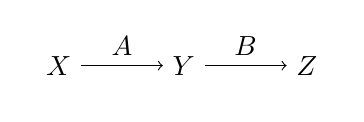
\begin{tikzpicture}
  \matrix (m) [matrix of math nodes, row sep=2em, column sep=3em, minimum width=1em]
  {
    X  & Y & Z  \\ };
  \path[->]
  (m-1-1) edge node [auto] {$A$} (m-1-2)
  (m-1-2) edge node [auto] { $B$} (m-1-3);
%  (m-2-1) edge node [below] {$\widetilde{A}$} (m-1-2);
\end{tikzpicture}

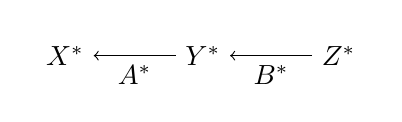
\begin{tikzpicture}
  \matrix (m) [matrix of math nodes, row sep=2em, column sep=3em, minimum width=1em]
  {
    X^*  & Y^* & Z^*  \\ };
  \path[->]
  (m-1-2) edge node [auto] {$A^*$} (m-1-1)
  (m-1-3) edge node [auto] { $B^*$} (m-1-2);
%  (m-2-1) edge node [below] {$\widetilde{A}$} (m-1-2);
\end{tikzpicture}


$(BA)^* : Z^* \to X^*$
\[
((BA)^* \zeta)(x) = \zeta(BAx) = (\zeta B)(Ax) = (B^* \zeta)(Ax) = (A^* B^*)\zeta(x)
\]

\item[(b)]
\[
(Id_V)^*(\nu(x)) = \nu(1x) = \nu(x)
\]
\end{enumerate}

\subsection*{ Tangent Covectors on Manifolds}



\subsection*{ The Cotangent Bundle}

\begin{proposition}[6.5] Let $M$ smooth manifold, $T^*M = \coprod_{p \in M} T_p^*M$ \\
with $\begin{aligned} & \quad \\
  & \pi : T^*M \to M \\
  & \omega \in T^*_pM \to p \end{aligned}$

natural vector space structure on each fiber, \\
$\exists \, !$ smooth manifold structure making $T*M$ rank-$n$ vector bundle over $M$, \\
s.t. all coordinate covectors are smooth local sections
\end{proposition}

\subsection*{ The Differential of a Function }



\end{document}
